\documentclass[t]{beamer}

%\documentclass[handout, t]{beamer}
\setbeamertemplate{navigation symbols}{}
\usepackage{pstricks}
\usepackage{mathtools}
\usepackage{amsfonts}
\usepackage{mathrsfs}
\usepackage{amsmath}
\setbeamertemplate{navigation symbols}{}
\usepackage{bm}
\usepackage[UTF8]{ctex}
\usetheme{AnnArbor}
\usefonttheme{serif}
\useinnertheme{rounded}
%\usecolortheme{crane}
\setbeamertemplate{blocks}[rounded][shadow=true]

\newcommand{\dif}{{\;\rm d}}
\usepackage{graphicx}
\usepackage{pgf}
\usepackage{tikz}
\usetikzlibrary{arrows, decorations.pathmorphing, backgrounds, positioning, fit, petri, automata}
\tikzset{>=stealth}
\usepackage{listings}


\lstset{
  language=Python, % 设置语言
  basicstyle=\ttfamily, % 设置字体族
  breaklines=true, % 自动换行
  keywordstyle=\bfseries\color{blue}, % 设置关键字
  ndkeywordstyle=\bfseries\color{blue}, % 设置关键字
  classoffset=0,
  emph=[0]{self, plt, pd, np, print, sm, None, True, False, Logit}, % 指定强调词,如果有多个,用逗号隔开
  emphstyle=\bfseries\color{magenta!90!black}, % 强调词样式设置
  classoffset=1,
  moreemph=[1]{plot, text, title, show, scatter, as, fit}, % 设置更多的关键字,用逗号分隔
  emphstyle=\bfseries\color{blue}, % 强调词样式设置
  classoffset=0,
  commentstyle=\itshape\color{gray}, % 设置注释样式,斜体,浅灰色
  stringstyle=\bfseries\color{green!50!black}, % 设置字符串样式
  columns=flexible,
  numberstyle=\footnotesize, % 缩小行号
}


\setmainfont{Times New Roman}
\setCJKmainfont{Microsoft YaHei}


\hypersetup{pdfpagemode=FullScreen}
\renewcommand{\Pr}{\mathbb{P}}
\usepackage{blkarray}


\setbeamercolor{block title}{bg=red!10!white}
\setbeamercolor{block body}{bg=gray!10!white}

\usepackage{multicol}
\newcommand{\E}{\mathbb{E}}
\newcommand{\EP}{\mathbb{E}^{\mathbb{P}}}
\newcommand{\EQ}{\mathbb{E}^{\mathbb{Q}}}
\newcommand{\Var}{{\rm Var}}
\newcommand{\Cov}{{\rm Cov}}


\begin{document}
\fontsize{11}{18}\selectfont


\CTEXindent



  \title{第四章~~银行业数据分析}
\author{方杰、李烜}
\date{福建江夏学院金融学院}
  \begin{frame}
    \maketitle
  \end{frame}

\begin{frame}{本章内容}

    \tableofcontents
\end{frame}

\section{银行经营绩效的线性回归分析}
\subsection{回归分析的概念和原理}
\begin{frame}    \frametitle{回归分析的概念}
  回归分析:确定两种或两种以上变量间相互依赖的定量关系的一种统计分析方法

  一元线性回归的数学模型
\[y=ax+b+\varepsilon\]

  多元线性回归的数学模型
  \[y=a_1x_1+a_2x_2+\cdots+a_nx_n+b+\varepsilon\]
\begin{multicols*}{2}
  \begin{itemize}
  \item $y$:因变量
\item $b$:常数项
  \item $\varepsilon$:误差项
  \item $x_i$:自变量($i=1,2,\ldots,n$)
  \item $a_i$:自变量系数($i=1,2,\ldots,n$)
\end{itemize}
\end{multicols*}


\end{frame}


\begin{frame}
    \frametitle{线性回归模型的原理}
    残差平方和SSE,用作衡量实际值与模型估计值的接近程度
    \[{\rm SSE}= \sum_i \left(y^{(i)}-\hat y^{(i)}\right)^2=\sum_i \left[y^{(i)}-\left(ax^{(i)}+b\right)\right]^2 \]

    最小二乘法(Least Squares)的目标是使得残差平方和最小,此时的$a$和$b$即为所求的线性回归模型回归系数和常数项。

    方法:对残差平方和求导,令导数为0,求解$a$和$b$  
\end{frame}

\subsection{线性回归模型的应用}
\begin{frame}
    \frametitle{线性回归模型的应用}
  线性回归的基本步骤:
\begin{itemize}
  \item  确定自变量和因变量
  \item  变量间相关性分析
\item  建立回归分析模型
\item  模型检验
\end{itemize}    

\end{frame}

\begin{frame}
    \frametitle{ 确定自变量和因变量}
\begin{itemize}
  \item 明确考察的具体目标——因变量
  \item 目标的相关影响因素——自变量
\end{itemize}
    

\end{frame}


\begin{frame}[fragile]
    \frametitle{变量间相关性分析}
回归分析:对具有因果关系的影响因素 (自变量)和考察对象(因变量)所进行的数理统计分
    析处理。当变量与因变量确实存在某种关系时,建立的回归方程才有意义。

    相关系数:变量间具有较高相关性,说明建立线性模型进行分析是具有实际意义的。

\[\rho_{X,Y}=\frac{{\rm Cov}(X,Y)}{\sigma_X \sigma_Y}=\frac{\E\left[(X-\mu_X)(Y-\mu_Y)\right]}{\sigma_X \sigma_Y}\]
\begin{block}{Python代码实现}
  \begin{lstlisting}
df.corr()     # 生成的结果是相关性矩阵
\end{lstlisting}  
\end{block}
  
\end{frame}


\begin{frame}[fragile]
    \frametitle{建立回归分析模型}
    \verb|statsmodels|库中的\verb|ols|函数可以建立回归分析模型
\begin{lstlisting}
import statsmodels.formula.api as sm
import pandas as pd
result = sm.ols('Y ~ X', dataset).fit()
\end{lstlisting}
\begin{itemize}
  \item   \verb|Y|: 指定线性回归的因变量
  \item \verb|X|: 指定线性回归的自变量
  \item \verb|dataset|: $Y$和$X$所在的DataFrame格式的数据
  \item \verb|fit()|: 用于对模型进行拟合
  \item \verb|result|: 模型结果,包括自变量的系数和常数项等。可以使用\verb|result.params|调用模型中的结果
\end{itemize}
\end{frame}

\begin{frame}[fragile]
  \frametitle{回归分析的结果}
  使用以下命令,可得到回归分析结果\verb|result|的表格
\begin{lstlisting}
  print(result.summary())
\end{lstlisting}
\normalsize
\begin{itemize}
  \item \verb|Dep. Variable|: 输出变量,因变量
  \item \verb|Model|: 使用的模型类型
  \item \verb|Method|: 模型求解方式
  \item \verb|No. Observations|: 观测值的数量
  \item \verb|Df Residuals|: 残差计算的自由度
  \item \verb|coef|: 回归系数,其中\verb|Intercept|为常数项(截距项)
  \item \verb|std err|:常数项和变量系数的估计标准差
  \item \verb|t|, \verb"P>|t|": 分别为常数项和变量系数的$t$统计量值,以及$t$检验下的$p$-value
  \item \verb|[0.025, 0.075]|: 95\%显著性水平下的置信区间
\end{itemize}

\end{frame}


\begin{frame}[fragile]
  \frametitle{回归分析的结果(cont.)}
\begin{itemize}
  \item  \verb|Skew|, \verb|Kurtosis|: 分别为残差的偏度和峰度,可以用来判断残差是否符合正态分布
  \item \verb|Durbin-Watson|: 判断残差是否一阶相关
  \item \verb|R-squared|: 拟合优度,取值越接近于1,表示拟合效果越好
  \item \verb|Adj. R-squared|: 通过样本数量和模型参数数量修正后的拟合优度
  \item \verb|F-statistic|, \verb|Prob(F-statistic)|: $F$统计量及原假设成立概率
  \item \verb|Log-Likelihood|: 对数极大似然估计
  \item \verb|AIC|, \verb|BIC|: 赤池信息准则和贝叶斯信息准则,用于判断最优模型
  \item \verb|Jarque-Bera(JB)|, \verb|Prob(JB)|: Jarque-Bera统计量及原假设成立概率,用于残差正态性的判断
\end{itemize}
  

\end{frame}

\begin{frame}[fragile]
  \frametitle{模型检验}
  为观察拟合效果,输入绘制代码:
\begin{lstlisting}
import matplotlib.pyplot as plt 
# 绘制散点图
plt.scatter(data['X'], data['Y'])
# 拟合线性回归图
plt.plot(data['X'], result.params[0] 
            + result.params[1]*data['X'], 'r') 
plt.text(1,3, 'y=' + str(round(result.params[1],4)) + '+'
            + str(round(result.params[0],4)) +'*x') 
plt.title('linear regression')
plt.show()
\end{lstlisting}

\end{frame}

\section{银行信贷风险的逻辑回归分析}
\begin{frame}[fragile]
  \frametitle{信贷风险评估}
商业银行信贷风险评估,主要是在客户
贷款之前,然而在发放信贷过程中或者
之后的风险,银行很难及时发现和控制,
需要客户在与银行发生业务过程记录的
信息来评价贷后风险,以利于及时作出
风险管控措施。
  

\end{frame}

\begin{frame}[fragile]
  \frametitle{信贷违约风险}
违约概率(Probability of default)是预计债务人不能偿还到期
债务(违约)的可能性。在实践中,银行会将违约概率对作为量
化信用风险的关键参数之一,并依此对用户分类。

在实践中,银行会将次级、可疑、损失三种类型列为信贷违约。
\end{frame}


\begin{frame}[fragile]
  \frametitle{传统违约概率计算模型}
\begin{itemize}
  \item CreditMetirics模型
  \item KMV模型
  \item Credit Risk模型
\end{itemize}
\begin{block}{传统风险度量方式弊端}
\begin{itemize}
  \item 模式只适用于经营管理、信息
记录规范的企业
\item 模型不全面,忽略了一些市
场风险,与市场真实情况存在一
定误差
\item 信息不对称,使用的公司数
据非实时,结果可靠性有限
\end{itemize}
\end{block}

\end{frame}


\subsection{信贷风险的
逻辑回归模型}
\begin{frame}[fragile]
  \frametitle{信贷风险的逻辑回归模型}

受限因变量模型(Limited Dependent Variable model, LDV),是一类因变量取值为二分类数据的特殊模型。常见的有Logit模型、Probit模型等。

  逻辑(Logistic)回归(Logit Regression)是目前银行建立大数据信用评估最常用的方法,可以解决二分类的
  非线性问题。
  
  在信用评估时,用逻辑回归模型返回的违约概率结果是0到1之间以小数形式呈现的类概率数
  字,用以判断客户是否会违约,以及违约的可能性大小,具有对特征可解释性强的优点。
\end{frame}

\begin{frame}[fragile]
  \frametitle{逻辑回归的数学模型}
假设线性回归模型
\[{\bf a}'{\bf x}+b = \begin{bmatrix}
  a_1&a_2&\cdots&a_n
\end{bmatrix}\begin{bmatrix}
  x_1\\x_2\\ \vdots \\x_n
\end{bmatrix}+b=a_1x_1+a_2x_2+\cdots+a_nx_n+b \]
然后使用一个单位阶跃函数,将结果映射到$[0,1]$。对于逻辑回归模型而言,该函数的形式如下:
{\LARGE\[ f\,({\bf x})=\frac{1}{1+e^{-({\bf a}'{\bf x}+b)}}\]}



\end{frame}

\begin{frame}[fragile]
  \frametitle{单位阶跃函数}
\begin{center}
  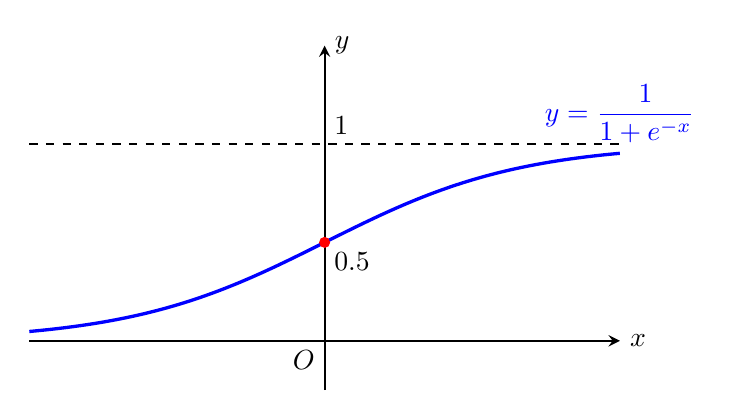
\begin{tikzpicture}[scale=1.25]
\draw[->, thick](-3,0)--(3,0)node[right]{$x$};
\draw[->, thick](0,-.5)--(0,3)node[right]{$y$};
\draw[dashed](-3,2)--(3,2);
\draw [domain=-3:3, samples=300, very thick, blue]plot(\x, {2/(1+exp(-\x))})node[above]{$y=\dfrac{1}{1+e^{-x}}$} ; 
\node at (0,0)[below left]{$O$};
\node at (0,2)[above right]{1};
\node at (0,1)[below right]{0.5};
\draw[fill, red](0,1)circle(.05);
  \end{tikzpicture}
\end{center}
\end{frame}  



\begin{frame}[fragile]{逻辑回归的数学模型(cont.)}
  将逻辑回归输出与二分类问题输出$y=\{0, 1\}$建立联系

  设0.5为临界值:
\begin{itemize}
  \item 当$f({\bf x})>0.5$,即${\bf a}'{\bf x}+b>0$时,$y$为1;
  \item 当$f({\bf x})<0.5$,即${\bf a}'{\bf x}+b<0$时,$y$为0;
  \item $f({\bf x})$越接近临界值0.5则无法判断,分类准确性下降。
\end{itemize}

\begin{block}{说明:}
  逻辑回归被广泛应用于分类问题,并且不要求自变量和因变量之间有线性关系。与线性回归模型相比,逻辑回归{\color{red}对异常值不敏感}
\end{block}
\end{frame}

\begin{frame}[fragile]{逻辑回归分析的Python实现}
Python中\verb|statsmodels|包的\verb|Logit|函数可以实现逻辑回归模型构建
\begin{lstlisting}
import numpy as np
from statsmodels.api import Logit
logit = Logit(yTrain, XTrain) 
# yTrain是因变量(取值为0或1)训练集;XTrain是自变量训练集
result = logit.fit()
print(result.summary())
\end{lstlisting}
\end{frame}

\begin{frame}[fragile]{逻辑回归分析的预测与检验}
用测试集进行预测,结果为事件发生的概率,取值在$[0,1]$之间。将预测结果与0.5进行比较,大于等于0.5,则判
定事件发生,取值为“1”;反之,判定事件不发生,取值为“0”
\begin{lstlisting}
import pandas as pd
pred = result.predict(XTest) 
# result是前面逻辑回归模型的拟合结果
Value = round(pred)  # 预测结果>=0.5的,判定为1;反之为0
compare = pd.DataFrame({'predictedValue':pred, 'roundValue':Value, 'actual':y.tail(10)})  # 引号中的是列名定义
print(compare)  # 这里y.tail(10)存储的是实际因变量取值
print(np.sum(Value==y.tail(10))/10)  # 计算10个预测值的准确率
\end{lstlisting}
\end{frame}


\end{document}